\section{以 "call-fs-mcp" Demo 为例介绍系统架构}
\bf{"call-fs-mcp"} 是一个基于 snowy 框架开发的 Demo 工程，用于演示\it{如何通过 MCP 接口将 Web 应用（WebApp）与 FS 仿真引擎集成}：前端页面发起仿真控制操作，后端通过 MCP \texttt{tools/call} 调用 FS 仿真引擎能力，仿真运行状态与动画通过 MQTT 实时回传，从而完成"模型加载 $\rightarrow$ 仿真运行 $\rightarrow$ 结果获取 $\rightarrow$ 动画展示"的完整闭环。本章以该 Demo 为例介绍系统逻辑架构、各模块功能与交互关系。

\subsection{系统逻辑架构}
系统逻辑架构如图\ref{fig:mcp-architecture}所示（\bf{各层之间通过标准接口解耦}）：
% \begin{figure*}[!h]
% 	\centering
% 	\resizebox{0.7\linewidth}{!}{\input{out/uml/mcp/architecture/architecture.latex}}
% 	\caption{系统逻辑架构图}\label{fig:architecture}
% \end{figure*}

\begin{figure}[H]%[htbp!]
	\centering
	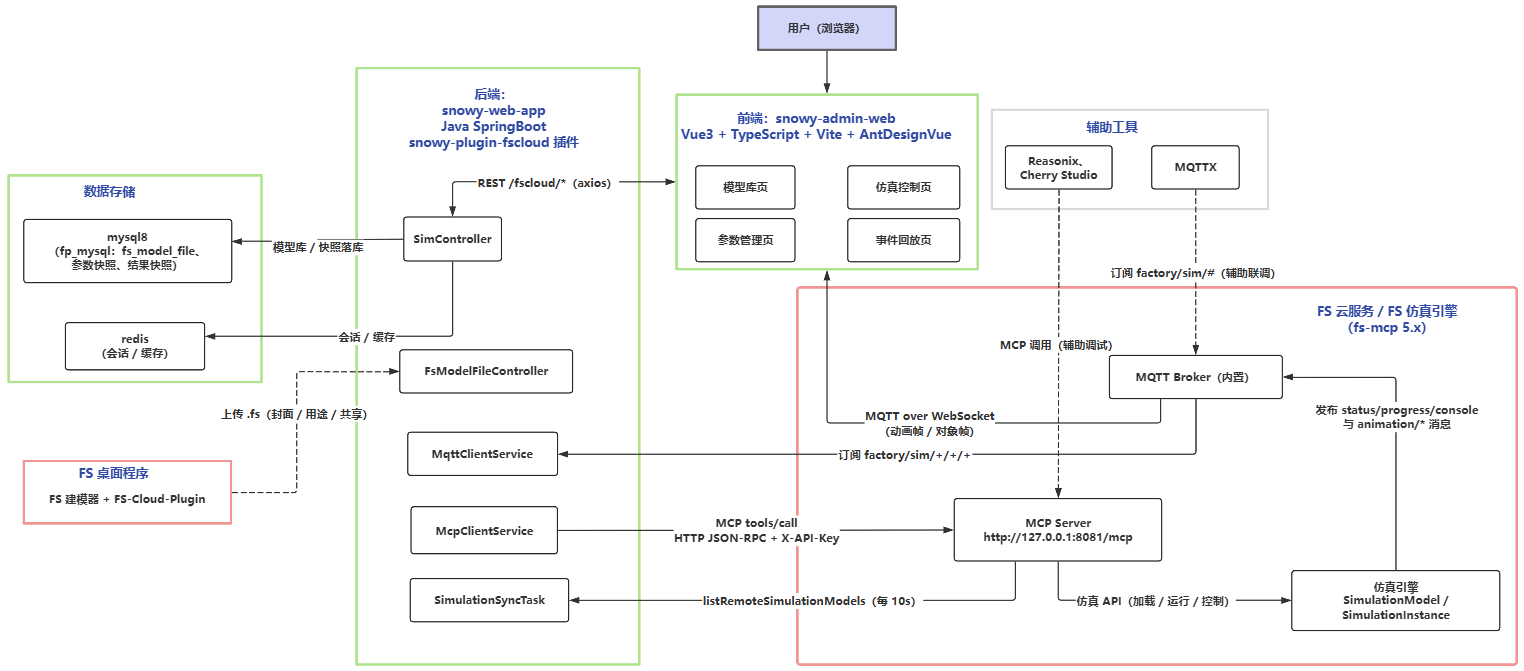
\includegraphics[width=1.0\textwidth]{pics/mcp/architecture.png}
	\caption{MCP 仿真工程架构}\label{fig:mcp-architecture}	
\end{figure}

数据存储：
\begin{itemize}
	\item \bf{mysql8}（库名 \texttt{fp\_mysql}）：保存模型库记录（\texttt{fs\_model\_file}）、参数快照（\texttt{fs\_sim\_param\_snapshot}）、结果快照、系统权限数据等。
	\item \bf{redis}：snowy 框架的会话/缓存基础设施（登录态、权限缓存等）。
\end{itemize}

\subsubsection{各模块的功能说明}
\begin{enumerate}[label=\arabic*)]
	\item \bf{前端（snowy-admin-web）}：snowy 框架的前端工程，\it{Vue3 + TypeScript + Vite + AntDesignVue}。主要页面与职责：
	\begin{itemize}
		\item \it{模型库页}：模型文件的上传展示、加载/卸载模型，调用 \texttt{/fscloud/modelfile/*} 与 \texttt{/fscloud/sim/loadModel}。
		\item \it{仿真控制页}：启动、暂停、恢复、停止、重置仿真，查询状态与结果快照，开关动画、调节加速因子，显示 MQTT 实时日志与动画画面。
		\item \it{参数管理页}：读取/编辑模型参数表，参数快照的保存、加载、删除与写回模型。
		\item \it{事件回放页}：按仿真时间轴滑动查询对象位置快照与时间窗仿真事件，订阅实时对象帧用于数据分析。
	\end{itemize}
	\item \bf{后端（snowy-web-app + snowy-plugin-fscloud）}：snowy 框架的后端工程，\it{SpringBoot + Java}。FS 集成业务集中在插件模块 \texttt{snowy-plugin-fscloud} 中：
	\begin{itemize}
		\item \texttt{SimController}：暴露 \texttt{/fscloud/sim/*} 仿真控制 REST 接口（加载、运行、暂停、恢复、停止、重置、卸载、状态、结果、参数、动画、时间轴分析等），带 \texttt{@SaCheckPermission} 权限校验。
		\item \texttt{FsModelFileController / FsModelFileService}：模型库的增删改查与上传（\texttt{/fscloud/modelfile/*}），处理 FS-Cloud-Plugin 上传的 \texttt{.fs} 文件：落盘到 \texttt{uploaded/\{userId\}/} 并落库 \texttt{fs\_model\_file}。
		\item \texttt{McpClientService}：MCP 客户端封装，通过 HTTP JSON-RPC 2.0（\texttt{X-API-Key} 鉴权）调用 FS 的 MCP Server，统一解包 \texttt{result.content[0].text} 业务 JSON。
		\item \texttt{MqttClientService}：Paho MQTT 客户端，订阅 \texttt{factory/sim/+/+/+}，把 \texttt{status/progress/console} 消息同步到内存记录与数据库。
		\item \texttt{SimulationSyncTask}：定时任务（每 10s）调用 \texttt{listRemoteSimulationModels}，同步内存 \texttt{SimulationModelTrackingMap} 与数据库中的模型状态。
	\end{itemize}
	\item \bf{FS 桌面程序（FS 建模器、仿真引擎）}：FS 建模器用于编辑 \texttt{.fs} 模型（含定义 \texttt{mcp} 参数表）；仿真引擎负责模型的编译与仿真运行。\it{在本方案中，FS 桌面程序亦可作为 FS 云服务的仿真引擎使用}（\texttt{loadInUI=true} 时把模型挂载到桌面 UI，方便人工观察）。
	\item \bf{FS-Cloud-Plugin（真实应用可选）}：FS 建模器的插件，用于把模型文件（\texttt{.fs}）上传到云端后端，可携带\it{封面图片、模型用途和共享设置}。Demo 中后端已支持其登录与上传协议。
	\item \bf{FS 云服务和接口（FS 仿真引擎）}：作为服务端运行，内部包含 \it{MCP Server}（HTTP JSON-RPC）与 \it{内置 MQTT Broker}。
	\item \bf{MCP 连接}：默认 \texttt{http://127.0.0.1:8081/mcp}。
	\item \bf{MQTT 连接}：后端 \texttt{tcp://localhost:1883}，前端 WebSocket \texttt{ws://127.0.0.1:8083/mqtt}。
	\item \bf{数据库}：\it{mysql8}（业务数据）+ \it{redis}（会话缓存）。
	\item \bf{辅助工具}：
	\begin{itemize}
		\item \it{MQTTX 客户端软件}：订阅 \texttt{factory/sim/\#} 监听 MQTT 消息，辅助应用开发调试（查看状态/进度/控制台/动画帧消息）。
		\item \it{Reasonix 或 Cherry Studio 桌面软件}：以问答方式直接调用 MCP 接口（\texttt{tools/list}、\texttt{tools/call}），辅助应用开发调试（需配置 MCP 端点与 API Key）。
	\end{itemize}
\end{enumerate}

\subsection{各模块之间的交互说明}
各模块的交互关系可归纳为三条主线：
\begin{enumerate}[label=\arabic*)]
	\item \bf{控制流（前端 $\rightarrow$ 后端 $\rightarrow$ FS）}：前端通过 REST 调用后端接口，后端 \texttt{SimController} 经 \texttt{McpClientService} 把请求转成 MCP \texttt{tools/call} 发给 FS MCP Server，FS 执行后在响应中返回结果，后端再回传给前端。\bf{前端不直接调用 MCP}，鉴权、跨域、API Key 等由后端统一处理。
	\item \bf{实时数据流（FS $\rightarrow$ MQTT Broker $\rightarrow$ 后端/前端）}：仿真运行期间，FS 引擎把 \texttt{status/progress/console} 和 \texttt{animation/*} 消息发布到内置 MQTT Broker；\it{后端与前端各自独立订阅、二者没有 MQTT 联系}。
	\item \bf{订阅主题}：后端 \texttt{MqttClientService}（Paho TCP）订阅 \texttt{factory/sim/+/+/+}（\it{所有用户所有模型}）并同步状态到数据库。
	\item \bf{前端订阅}：前端（WebSocket + mqtt.js）订阅 \texttt{factory/sim/\{userId\}/\{modelId\}/\#}（\it{当前用户当前模型}），接收动画帧与结构化对象帧用于展示。
	\item \bf{模型数据流（FS-Cloud-Plugin $\rightarrow$ 后端 $\rightarrow$ 数据库）}：FS 建模器通过 FS-Cloud-Plugin\secref{appendix:plugin}登录后端并上传 \texttt{.fs} 模型文件，后端落盘后写入 \texttt{fs\_model\_file}，形成模型库；仿真控制时后端按记录拼出模型文件绝对路径传给 \texttt{loadRemoteSimulationModel}。
\end{enumerate}

\subsection{MCP 接口在系统中的调用流程}
一次"启动仿真"的 MCP 调用流程示意如下（其余控制类工具流程相同）：
\begin{verbatim}
前端（仿真控制页"启动"按钮）
   |
   |  POST /fscloud/sim/runModel { id, modelId, showAnimation }
   v
后端 SimController.runModel
   |  userId = StpUtil.getLoginIdAsString()
   |  McpClientService.startSimulation(userId, modelId, showAnimation)
   |     构造 { jsonrpc:"2.0", method:"tools/call",
   |            params:{ name:"startRemoteSimulation", arguments:{...} } }
   |  HTTP POST http://127.0.0.1:8081/mcp（X-API-Key）
   v
FS MCP Server
   |  RemoteSimulationTools.startRemoteSimulation
   |   -> RemoteSimulationManager 校验配额/生成 runId/保存参数快照
   |   -> SimulationRunningThread 启动仿真线程
   |  返回 { success:true, data:{ runId, status:"RUNNING", ... } }
   v
后端 McpClientService
   |  解包 result.content[0].text -> 业务 JSON
   |  更新 SimulationModelTrackingMap + 写回 fs_model_file.sim_status
   v
前端（响应体展示状态卡片，MQTT 持续推送进度/日志）
\end{verbatim}
\vspace{-30pt}
要点：
\begin{itemize}
	\item MCP 响应是\it{两层结构}：先解析 JSON-RPC 响应取 \texttt{result.content[0].text}，再解析该字符串得到统一业务 JSON（\texttt{success}、\texttt{code}、\texttt{message}、\texttt{data}）。
	\item 工具定位参数：\texttt{userId}（来自后端登录态）+ \texttt{modelId}（\texttt{loadRemoteSimulationModel} 返回并落库，前端仅透传）。
	\item 控制类调用为\it{请求-响应}式；运行过程中的实时状态由 MQTT 通道推送，两者互补。
\end{itemize}

\subsection{前端与后端的交互流程}
前端与后端之间通过 \bf{REST（axios）}进行\it{请求-响应}式交互；实时消息由 FS 内嵌 MQTT Broker 广播，\bf{前端与后端各自独立订阅、两者之间没有 MQTT 联系}。

图\ref{fig:flowcharFEnBE}为\it{前端与后端的交互流程}

\begin{figure*}[!h]
	\centering
	\resizebox{1.0\linewidth}{!}{\input{out/uml/mcp/flowcharFEnBE/flowcharFEnBE.latex}}
	\caption{前端与后端的交互流程}\label{fig:flowcharFEnBE}
\end{figure*}

说明：
\begin{itemize}
	\item \bf{REST 通道}（前端 $\leftrightarrow$ 后端，请求-响应）：页面初始化恢复当前模型、加载/运行/暂停/停止/重置/卸载、参数表/结果快照/时间轴分析等查询；后端经 \texttt{SimController} $\rightarrow$ \texttt{McpClientService} $\rightarrow$ MCP 处理后将统一业务 JSON 返回前端。
	\item \bf{MQTT 通道}（FS 广播，前端与后端各自订阅、互不联系）：
	\begin{itemize}
		\item 后端 \texttt{MqttClientService}（Paho，TCP）订阅 \texttt{factory/sim/+/+/+}，覆盖\it{所有用户所有模型}，把 \texttt{status/progress/console} 同步到内存记录与数据库（\texttt{fs\_model\_file.sim\_status}）。
		\item 前端（mqtt.js，WebSocket）订阅 \texttt{factory/sim/\{userId\}/\{modelId\}/\#}，只接收\it{当前用户当前模型}的消息：状态/进度/控制台（JSON）与动画帧（JPEG）/对象帧（JSON）。
	\end{itemize}
	\item 前端状态轮询（\texttt{getRemoteSimulationStatus}）建议 1--2 秒间隔；动画帧由 MQTT 按帧率（默认 5 FPS）推送。
	\item 前端 API 统一封装在 \texttt{src/api/fscloud/fsSimApi.js}（\texttt{/fscloud/sim/*}）与 \texttt{fsModelFileApi.js}（\texttt{/fscloud/modelfile/*}）；实时模型状态保存在 Pinia store（\texttt{myModel.js}）。
\end{itemize}

